% CVPR 2027 submission. Build: tectonic main.tex (from paper/tex); supplementary alone: tectonic supp.tex
\documentclass[10pt,twocolumn,letterpaper]{article}
% !TEX root = main.tex
% Shared preamble: packages, macros and conference identifiers. Input by main.tex and supp.tex after their
% \documentclass line (kept out of this file so that Overleaf's main-document detection picks main.tex).

\usepackage[review]{cvpr}
\usepackage[T1]{fontenc}
\usepackage{times}
\usepackage{graphicx}
\usepackage{amsmath,amssymb}
\usepackage{booktabs}
\usepackage{multirow}
\usepackage{xcolor}
\definecolor{cvprblue}{rgb}{0.21,0.49,0.74}
\usepackage{colortbl}
\usepackage{enumitem}
\usepackage{microtype}
\renewcommand{\arraystretch}{0.93}
\setlength{\textfloatsep}{8pt}
\setlength{\abovecaptionskip}{4pt}
\makeatletter
\renewcommand\paragraph{\@startsection{paragraph}{4}{\z@}{1.5ex \@plus .5ex \@minus .2ex}{-1em}{\normalfont\normalsize\bfseries}}
\makeatother
\usepackage[pagebackref,breaklinks,colorlinks,citecolor=cvprblue,linkcolor=cvprblue,urlcolor=cvprblue]{hyperref}

\def\confName{CVPR}
\def\confYear{2027}
\def\paperID{XXXX}

\graphicspath{{figures/}}
\definecolor{tbd}{RGB}{176,96,0}
\definecolor{tbdbg}{RGB}{255,246,230}
\newcommand{\tbd}[1]{\colorbox{tbdbg}{\textcolor{tbd}{\footnotesize pending: #1}}}
\newcommand{\cur}{\textsc{cur}}
\newcommand{\curerr}{\textsc{cur-err}}
\newcommand{\auroc}{\textsc{auroc}}
\newcommand{\absrel}{\textsc{AbsRel}}
\newcommand{\bench}{HalluBench-3D}
\newcommand{\ci}[3]{#1\,{\scriptsize[#2,\,#3]}}


\title{Observe, Imagine, Abstain:\\Detecting Hallucinated Geometry in Feed-Forward 3D Reconstruction}

\author{Anonymous \confName~submission\\Paper ID \paperID}

\begin{document}
\maketitle

\begin{abstract}
Feed-forward 3D foundation models reconstruct a scene from unposed photographs in one pass. Where no photograph shows a surface, they fill the gap from learned priors and report the invented geometry with the confidence of an observed one. We define a predicted point as \emph{hallucinated} when it lies on a surface no input view observes, and build \bench{} to measure it: a 3D region of the ground-truth surface is hidden in every input view, so pixels inside it are unsupported and pixels far from it are supported. Across five models (VGGT, Pi3, Pi3X, MapAnything, Depth Anything 3), 18 DTU scans and 18 CO3Dv2 scenes, native confidence lets 24\% to 81\% of unsupported pixels through a threshold that keeps 90\% of supported ones (blur and noise fills; the gray fill goes down to 0.053). A matched split then shows what the confidence reads: when the same patch is hidden in some views but left visible in another, native confidence cannot tell it from the imagined one (\auroc{} 0.43 to 0.55 on DTU, 0.48 to 0.50 on CO3Dv2) and lets 80\% to 87\% of the imagined pixels through. It detects the patch, not the missing support. The information exists in the model: a linear probe on its cross-view tokens separates single-view from supported geometry at \auroc{} 0.99 where native confidence scores 0.8. A small \emph{support head} trained on the backbone's own multi-view agreement, with no ground truth, reads that signal on four backbones and four datasets it never saw (\auroc{} 0.93 to 0.99 against 0.55 to 0.89 for native confidence), matches a ground-truth-trained head within 0.02 and beats reprojection consistency on three datasets at a fraction of its cost; trained on the matched split, it separates the imagined patch from the observed one at \auroc{} 0.69 to 0.75 while its per-image twin stays at 0.56 to 0.61. Two cautions: a head trained on the benchmark's fills learns the fill, and no detector fires on a surface the model invents consistently in every view; what moves that surface is the pixels it was drawn from. Code, benchmark, heads and the full run log will be released.
\end{abstract}

%------------------------------------------------------------------------
\section{Introduction}
\label{sec:intro}

\begin{figure*}[t]
\centering
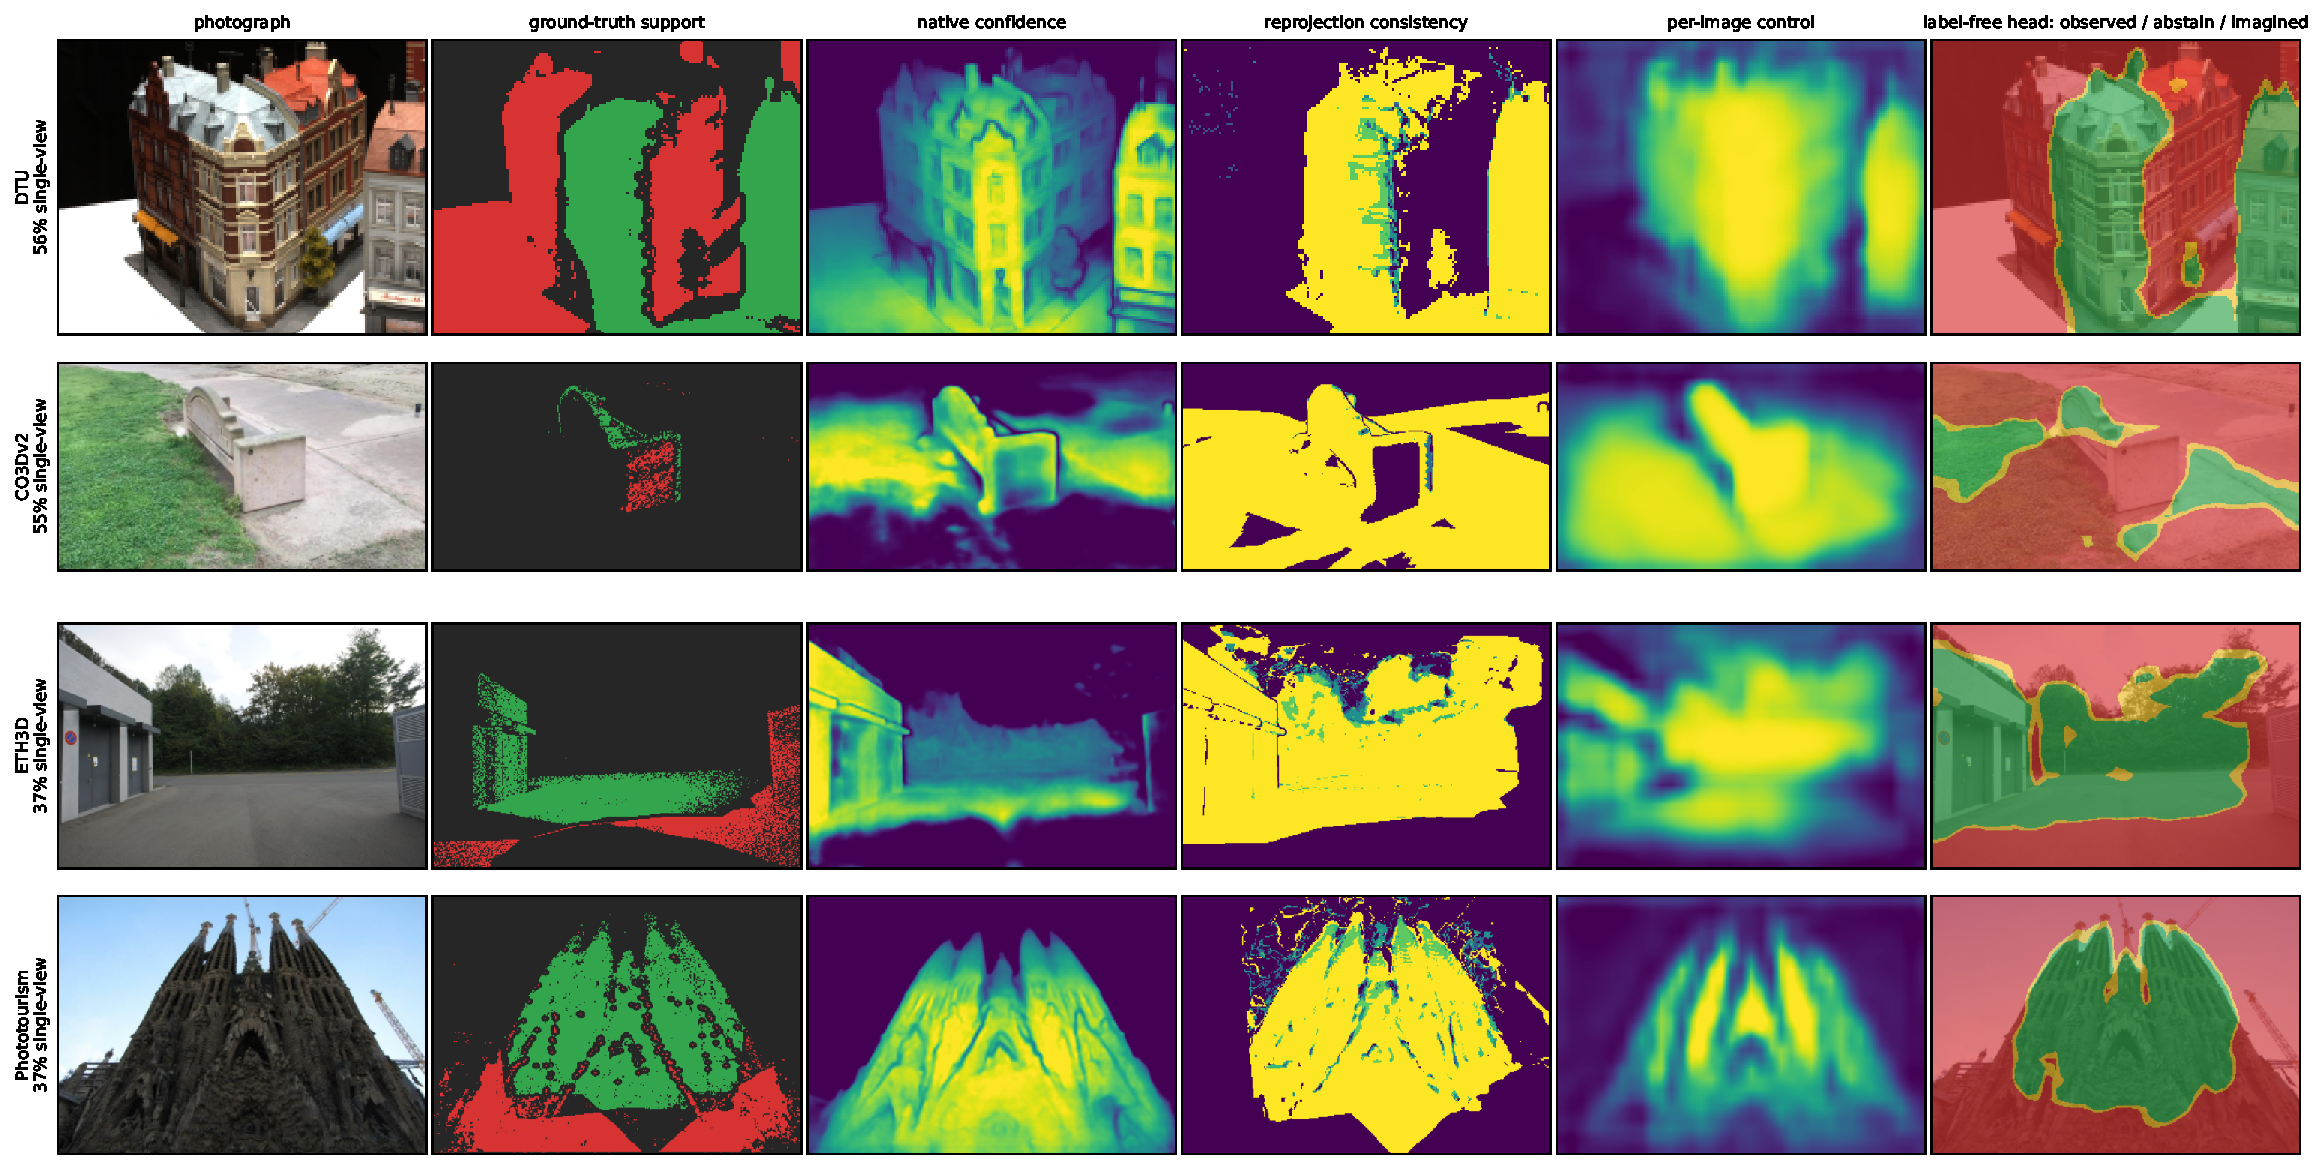
\includegraphics[width=0.74\textwidth]{fig_qual}
\caption{\textbf{What the label-free head says, on four captures it never saw.} One clean multi-view input per dataset (DTU rig, CO3Dv2 phone orbit, ETH3D DSLR, a tourist photograph of the Sagrada Fam\'ilia); ground-truth support (red: no other view sees the surface; green: two or more do; dark: no ground truth); VGGT's native confidence; reprojection consistency with its own cameras; the per-image control; the head's bands at the fixed thresholds (green observed, yellow abstain, red imagined). The head's labels came from the backbone's own predictions on DTU training scans; where native confidence lets half of the single-view pixels through a threshold that keeps 90\% of the supported ones on DTU, the head lets 1.7\% through. Run P6-dump.}
\label{fig:qual}
\end{figure*}

Feed-forward 3D reconstruction has moved from pairwise pointmaps~\cite{dust3r,mast3r} to models that take dozens of unposed images and return dense geometry in one pass~\cite{vggt,pi3,mapanything,da3}. They output geometry at every pixel, including pixels whose true surface no input view shows; the objective rewards a plausible guess, so they learn to guess, and the confidence map, the one signal a user has, does not say which parts were observed and which were guessed.

A conservator looking at a reconstruction of a dome sees a crack. Before sending someone up a scaffold, they want to know whether any photograph shows it or the model drew it from what domes look like; today the confidence map is bright in both cases.

We make three contributions.

\begin{enumerate}[leftmargin=*,itemsep=1pt,topsep=2pt]
\item \textbf{A definition, a benchmark, and the control that makes it clean.} We define hallucinated geometry as predicted points on surfaces that no input view shows. \bench{} produces these labels by 3D-consistent masking of ground-truth surfaces, with controls on the same pixels under clean input, and reports \auroc, \cur{} and \curerr{} for five models on DTU and CO3Dv2, three fill types, an inpainted fill and stress tests, each with cluster-bootstrap intervals and paired permutation tests. Its \emph{matched split} hides identical patches that another view does see: native confidence cannot tell them from the imagined ones (\auroc{} 0.43 to 0.55 on DTU), so a per-image or matched control is a required test for any detector of unobserved geometry, the shipped confidence included.
\item \textbf{The backbone already knows, and a label-free way to read it.} Multi-view support is linearly decodable from the second half of the backbone's cross-view layers and absent from its per-image tokens; a linear probe gets within 0.015 of any head we trained. We read that signal with a small head whose labels come from the backbone's own prediction, so it trains on any capture with no ground truth, and abstains in between. On four backbones and four datasets it never saw it passes two pre-registered tests against native confidence, a per-image control and a ground-truth-trained head (Section~\ref{sec:exp}), and trained on the matched split it reads cross-view evidence where its per-image twin cannot (0.69 to 0.75 against 0.56 to 0.61 \auroc). Trained on the benchmark's synthetic fills instead, it learns the fill, a warning for masking-based supervision.
\item \textbf{The limit, and where the invented surface comes from.} A surface the model invents consistently in every view passes every cross-view test we have, this head included, and five models of three families invent the same one. What moves it is the pixels it was drawn from: refilling the hidden region moves the invented surface (\auroc{} 0.82 to 0.98 against supported geometry), so the invention is read from the hole, not fixed by the prior.
\end{enumerate}

Every number comes from a logged run with a run id; the pass conditions of Sections~\ref{sec:results} and \ref{sec:exp} were written down, with dates, before the runs they judge (supplement). The headline claim we test, not assume, is that native confidence fails to flag unsupported geometry across current models. It holds, and the matched split says why: the confidence reads the patch, not the missing support.

%------------------------------------------------------------------------
\section{Related work}
\label{sec:related}

\paragraph{Feed-forward 3D reconstruction.}
DUSt3R and MASt3R~\cite{dust3r,mast3r} predict pointmaps for image pairs; VGGT~\cite{vggt}, Pi3 and Pi3X~\cite{pi3}, MapAnything~\cite{mapanything}, VGGT-Omega~\cite{vggtomega} and Depth Anything 3~\cite{da3} extend this to many unposed views in one pass. Each exposes a per-pixel confidence trained as a loss weight on observed data; none is trained to tell observed from unobserved surfaces. Pi3X replaces Pi3's near-binary confidence with continuous quality levels; MapAnything also offers a multi-view consistency confidence, a baseline below.

\paragraph{Hallucination in feed-forward 3D.}
Bratulic et al.~\cite{bratulic2025} show that attention heads of DUSt3R, VGGT and DA3 keep matching correspondences after small patches are occluded; they measure attention and Sampson error on ShapeNet pairs, not confidence or 3D labels. Paul et al.~\cite{paul2026} benchmark hallucination at the input level (unrelated scenes, repeated images, noise), scored by COLMAP consistency. 3D-Mirage~\cite{mirage} studies monocular depth under illusions; Li et al.~\cite{widerviews} show that wide viewpoint spans produce unsupported geometry, and Dadajonov and Umarhojiyev~\cite{sharperframes} that unobserved parts of a room escape inference-time uncertainty; neither has per-point labels. FreeInpaint~\cite{freeinpaint} fills masked regions on purpose, the mechanism these models apply unasked. Our definition is per point, with exact labels, and tests whether native confidence separates them.

\paragraph{Uncertainty for feed-forward 3D.}
ReVar3R~\cite{revar3r} takes per-point variance over perturbed runs; it beats native confidence on AUSE but, by its authors' account, misses stable systematic bias, which a confidently filled region is. Trust3R~\cite{trust3r} fits an evidential head on a frozen backbone, GeoCond~\cite{geocond} adds pose-level uncertainty, and Deng et al.~\cite{deng2026} find the implied uncertainty of seven backbones at least $2.4\times$ too small. All score uncertainty against ground-truth error, which conflates confident errors on observed surfaces with confident predictions on unseen ones; \cur{} isolates the second case. Closest to our detector, a linear probe on frozen VGGT features predicts \emph{camera-pose} failure (AUROC 0.935 against 0.797 for native confidence~\cite{vggtknows}) and a small head on the same features predicts pairwise co-visibility~\cite{covggt}; our support head is the dense, per-pixel analogue for unobserved \emph{geometry}, trained with no label at all, and the linear probe is one of our controls.

\paragraph{Generative and multi-sample 3D.}
Z3D~\cite{z3d} decodes hidden surfaces from frozen VGGT features, evidence that unobserved geometry is present in them. Feed-forward Gaussian splatting~\cite{anysplat} and ReconSplat~\cite{reconsplat}, which extrapolates beyond the observed views by design, and world models with a persistent Gaussian memory~\cite{l3gworld} store imagined and observed surfaces alike, where a per-point support signal belongs. VolFill~\cite{volfill} finds sample variation $1.3\times$ larger in occluded regions and diffusion depth ensembles~\cite{marigold,perfectingdepth} give sample-disagreement uncertainty; a generative head over quantized geometry~\cite{ursa,fsq} is the natural successor to our discriminative one.

\paragraph{Hallucination in vision-language models.}
POPE~\cite{pope} labels statements unsupported by the image; ours is the geometric analogue, geometry unsupported by any view.

%------------------------------------------------------------------------
\section{Defining geometric hallucination}
\label{sec:def}

Given input views $I_1,\dots,I_N$, a model returns for each view $i$ a depth map $D_i$ and a confidence map $C_i$. A pixel $p$ in view $i$ is \emph{supported} if its ground-truth surface point is visible in at least one input view, and \emph{unsupported} if it is visible in none. A model hallucinates at $p$ when it outputs geometry at an unsupported $p$ with high confidence.

\paragraph{Why confidence is the wrong tool.}
Native confidence is trained as a per-pixel loss weight on observed data, low where the target is noisy and high where it is smooth, so a region no view sees and the prior fills smoothly receives high confidence by construction; Section~\ref{sec:results} measures the effect.

\paragraph{Metrics.} Computed per (model, scene, seed, radius, fill), averaged with cluster-bootstrap intervals over scenes; pixels whose confidence ties with $\tau$ count as kept, so a near-binary confidence (Pi3) is not favoured.
\begin{itemize}[leftmargin=*,itemsep=1pt,topsep=2pt]
\item \auroc: $P(C_S > C_U)$ with ties counted half. 1.0 means every supported pixel outranks every unsupported one; 0.5 means confidence carries no information about support.
\item \cur: choose $\tau$ so that 90\% of supported pixels have $C\ge\tau$; \cur{} is the fraction of unsupported pixels with $C\ge\tau$, the hallucination rate after filtering by confidence.
\item \curerr: the fraction of unsupported pixels above $\tau$ whose \absrel{} exceeds 0.1. Confident and wrong.
\item $\absrel_U$, $\absrel_S$: depth error on unsupported and supported pixels after median scaling on supported pixels; controls: the same pixels under clean input and the ratio of median confidence inside the hidden region to its clean value.
\end{itemize}

%------------------------------------------------------------------------
\section{\bench}
\label{sec:bench}

\paragraph{Protocol.}
For each scene we take 10 views. A sphere is centred on a random ground-truth surface point in the reference view, with radius 0.10 or 0.18 of the object's bounding-box diagonal, resampled until it covers 2 to 35\% of the reference view. Every pixel in every view whose ground-truth point lies inside the sphere is hidden (the protocol figure in the supplement). Hidden pixels are filled with gray, a blur of the original, uniform noise, or an inpainting of the surround~\cite{telea}; the fill is an ablation so that results are not an artefact of a visible patch. Labels: U is hidden in all views; S is valid and outside a 6-pixel dilation of the hidden region; the ring in between is ignored. Five mask seeds per scene; masks are deterministic in (scene, seed, radius).

\paragraph{The matched split.}
Every unsupported pixel above sits under a filled patch and no supported pixel does, so a confidence that merely reacts to a patch would look as if it knew about missing support. The matched split removes the confound: three spheres of one radius and fill, matched in reference-view area, depth and local texture. Sphere A is hidden in every view, so its pixels are \emph{imagined} (U); sphere B is hidden in every view but an evidence set of one, two or half the views, so its filled pixels in the hidden views are \emph{observed} (S$_m$) wherever a clean view sees their ground-truth point; sphere D is hidden only in the evidence views, so every view carries two patches and counting patches cannot tell A from B. From a single image the patches are identical; only cross-view evidence separates them. \auroc$_m$ and \cur$_m$ score U against S$_m$, the \emph{patch reaction} scores clean S against S$_m$ (the drop under a patch that hides nothing), and S$_m$ is bucketed by evidence: one clean view at low or high parallax, two, three or more. Seeds 0 and 1, radius 0.18, three fills (run P11-matched).

\paragraph{Datasets.}
\emph{DTU}~\cite{dtu}: the 18 scans of the MVSNet validation split, 10 views spread over the 49-camera rig, input $420\times518$. \emph{CO3Dv2}~\cite{co3d}: 18 scenes, the two depth-carrying sequences of each of nine categories (apple, ball, bench, hydrant, mouse, teddybear, toytrain, toytruck, vase) from the single-sequence subset, with the official COLMAP depth as ground truth. The 10 views are spread over the full orbit; frames are $640\times360$ phone video, models run at $518\times294$ (or the transpose), and every threshold is unchanged from DTU. \emph{ETH3D}~\cite{eth3d}: nine DSLR building-scale scenes with laser-scanner ground truth ($640\times427$, models $518\times350$), the reference frame and its nine most co-visible frames. \emph{Phototourism}~\cite{imc2020}: nine landmarks of the Image Matching Challenge 2020 set (supplement): Internet photographs with people in front of the monument, unordered viewpoints and focal lengths, COLMAP depth as ground truth; per landmark the best-connected photograph and its 19 most co-visible neighbours at $640\times448$. ETH3D and the landmarks are used only by the true-visibility protocol of Section~\ref{sec:exp}, which draws its own view sets (3, 5 and 10 clean views, three rotations) on every dataset. Training-data overlap: VGGT, Pi3/Pi3X and Depth Anything 3 list CO3Dv2 among their training sets~\cite{vggt,pi3,da3}, MapAnything does not~\cite{mapanything}, and none lists DTU or ETH3D, so CO3Dv2 is in-distribution for three backbones and DTU and ETH3D out of distribution for all.

\paragraph{Models.}
VGGT-1B~\cite{vggt} (depth and depth confidence), Pi3 and Pi3X~\cite{pi3} (local point $z$ and sigmoid confidence), MapAnything~\cite{mapanything} (image-only metric mode), and Depth Anything 3~\cite{da3} (Large 1.1). Same views and resolution for all; fp16 on a T4. AnySplat~\cite{anysplat}, a feed-forward Gaussian-splatting model scored on each pixel's Gaussian depth with its opacity as confidence, is in the supplement from a partial run: the representation does not change the answer.

\paragraph{Statistics.}
Means carry 95\% cluster-bootstrap intervals over scenes (10,000 resamples); pairwise comparisons use a paired sign-flip permutation test on per-scene means (20,000 permutations), Holm-corrected within each family; its smallest $p$ is $0.00005$, written $p<0.0001$.

%------------------------------------------------------------------------
\section{Results on \bench}
\label{sec:results}

\begin{table*}[t]
\centering
\caption{\textbf{Native confidence leaks, on the lab rig and on phone captures.} Five models, full configuration (18 scenes $\times$ 5 mask seeds $\times$ 2 radii), pooled over the blur and noise fills; mean [95\% cluster-bootstrap CI over scenes]. \emph{conf ratio}: median confidence inside the hidden region over its clean value. \auroc$_m$, \cur$_m$: the matched split of Section~\ref{sec:matched}, the imagined patch against an identical filled patch that another view sees (seeds 0 and 1, radius 0.18; run P11-matched). Per-fill tables and intervals in the supplement. Runs P1-full, P2-full, P2-co3d, P2-co3d-b.}
\label{tab:dtu}
\footnotesize
\setlength{\tabcolsep}{3pt}
\resizebox{\textwidth}{!}{% generated by scripts/make_tab_leak.py (compact body version; intervals in tab_leak_full.tex)
\begin{tabular}{l cc >{\columncolor{matchbg}}c >{\columncolor{matchbg}}c cc >{\columncolor{matchbg}}c >{\columncolor{matchbg}}c}
\toprule
 & \multicolumn{4}{c}{DTU (lab rig)} & \multicolumn{4}{c}{CO3Dv2 (phone)} \\
\cmidrule(lr){2-5}\cmidrule(lr){6-9}
 & \multicolumn{2}{c}{vs clean} & \multicolumn{2}{c}{\cellcolor{matchbg}vs observed patch} & \multicolumn{2}{c}{vs clean} & \multicolumn{2}{c}{\cellcolor{matchbg}vs observed patch} \\
model & \auroc$\uparrow$ & \cur$\downarrow$ & \auroc$\uparrow$ & \cur$\downarrow$ & \auroc$\uparrow$ & \cur$\downarrow$ & \auroc$\uparrow$ & \cur$\downarrow$ \\
\midrule
VGGT-1B & 0.90 & 0.24 & 0.55 & 0.80 & 0.68 & 0.65 & 0.49 & 0.85 \\
Pi3 & 0.91 & 0.28 & 0.49 & 0.83 & 0.89 & 0.27 & 0.49 & 0.81 \\
Pi3X & 0.81 & 0.53 & 0.47 & 0.87 & 0.73 & 0.57 & 0.50 & 0.81 \\
MapAnything & 0.74 & 0.62 & 0.51 & 0.84 & 0.58 & 0.81 & 0.49 & 0.84 \\
Depth Anything 3 & 0.71 & 0.70 & 0.43 & 0.85 & 0.62 & 0.80 & 0.48 & 0.84 \\
\bottomrule
\end{tabular}
}
\end{table*}

\subsection{DTU: native confidence leaks}
\label{sec:dtu}

Table~\ref{tab:dtu} pools the full DTU configuration over the two natural-statistics fills, blur and noise (per-fill tables in the supplement; the gray fill, which every model sees as a patch, gives the smallest numbers, down to \cur{} 0.053 for Pi3): \cur{} is 0.242 for VGGT, 0.281 for Pi3, 0.532 for Pi3X, 0.622 for MapAnything and 0.701 for Depth Anything 3, with \auroc{} 0.903, 0.912, 0.813, 0.743 and 0.711. Three tiers emerge. VGGT and Pi3 drop their confidence inside the hidden region (to 19 to 41\% of its clean value) yet let one in four unsupported pixels through; Pi3X leaks one in two and under a noise fill is as confident about geometry it cannot see as about geometry it can (ratio 1.09); MapAnything and Depth Anything 3 are close to blind, DA3's confidence inside the hidden region staying at 80 to 86\% of its clean value.

Pairwise, after Holm correction: VGGT and Pi3 are indistinguishable ($p=0.41$) and both leak less than the other three ($p\le0.0015$); Pi3X, MapAnything and DA3 are not separated from one another (supplement).

\paragraph{Confident and wrong.}
On DTU the imagined depth is accurate for four of the five models ($\absrel_U$ 0.011 to 0.022, about 1.3 to $2\times$ the clean value), so \curerr{} stays near zero. The failure is that you cannot tell imagined from observed, not that the imagination is poor; MapAnything is the exception, with 29\% of its unsupported pixels confident and wrong by more than 10\% \absrel{} on top of a 10\% error on supported pixels. The pass condition fixed before the benchmark was scaled (\cur{} above zero, \auroc{} clearly below one on the natural fills) holds for all five models.


\subsection{What the confidence reads: the matched split}
\label{sec:matched}

\begin{figure*}[t]
\centering
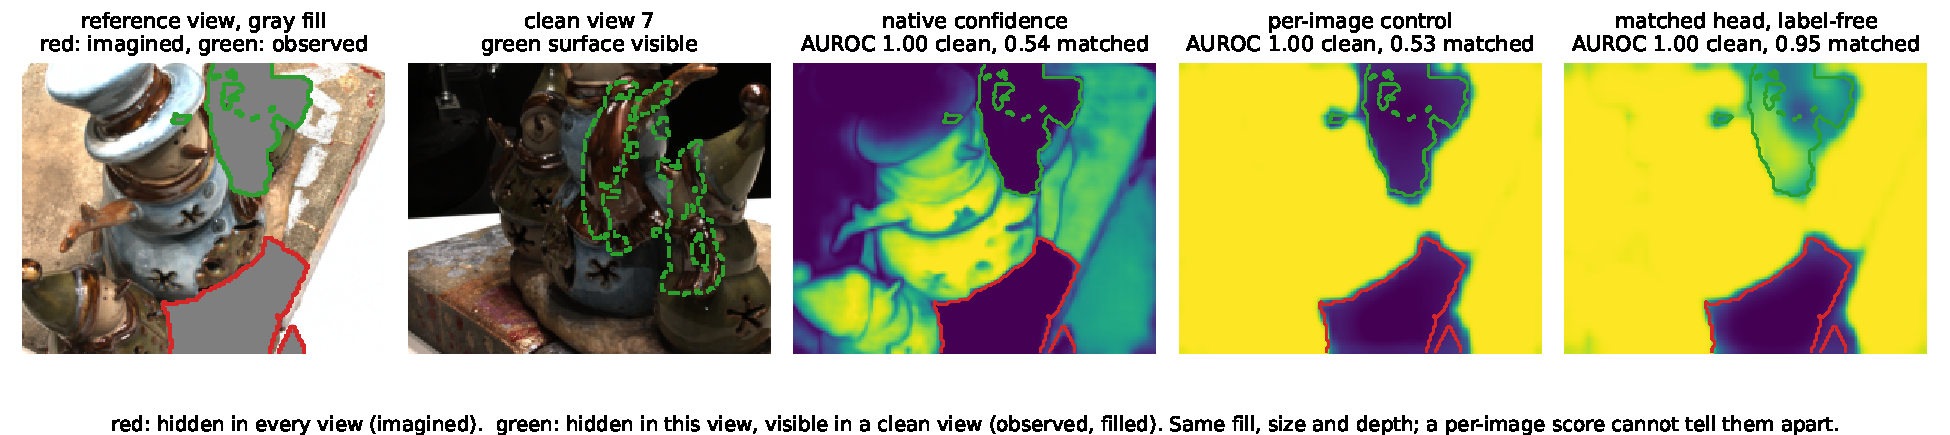
\includegraphics[width=0.86\textwidth]{fig_matched}
\caption{\textbf{Same patch, two labels.} Two identical gray patches on a DTU scan: red is hidden in every input view (imagined), green is hidden here but visible in the clean view beside it (observed). Native confidence and the per-image control score both alike; the matched head, trained label-free, separates them. Titles: each detector's \auroc{} on this scene against clean pixels and against the observed patch. Run P11-matched.}
\label{fig:matched}
\end{figure*}

The matched columns of Table~\ref{tab:dtu} and Figure~\ref{fig:matched} put the five models on the matched split. Against clean pixels native confidence separates the imagined patch at \auroc{} 0.72 to 0.94. Against an identical patch that another view does see, it separates nothing: \auroc$_m$ 0.43 to 0.55, at chance for every model, and \cur$_m$ 0.80 to 0.87: a threshold that keeps 90\% of the filled-but-observed pixels keeps 80\% to 87\% of the imagined ones. The patch reaction is 0.75 to 0.92: the original \auroc{} is the confidence dropping under a patch, whichever label the patch carries. On CO3Dv2 the same holds: \auroc$_m$ 0.48 to 0.50 against 0.58 to 0.90 for clean pixels, \cur$_m$ 0.81 to 0.85. The reprojection test with the model's own cameras is at chance on the matched pixels too (0.43 to 0.50): the invented surface is cross-view consistent. Gate 6 (supplement) called a model \emph{patch-inflated} when the matched \auroc{} fell more than 0.10 below the original; it falls 0.24 to 0.43 for the five, so Table~\ref{tab:dtu} is a lower bound and \cur$_m$ is the number to read: native confidence does not know what the model has seen; it reacts to the look of a patch.

\subsection{Stress tests, phone captures, cheap detectors}
\label{sec:stress}

The stress table in the supplement bounds the effect of the patch's appearance four ways. An inpainted fill, edge-continuous and without texture discontinuity, raises leakage further for VGGT ($+0.088$, $p=0.031$) and Pi3X ($+0.068$, $p=0.005$): Table~\ref{tab:dtu} is a lower bound for a natural-looking occluder. Dropping from 10 to 3 views leaves \cur{} unchanged for VGGT and Pi3X ($p>0.4$; DA3 moves at 5 views, $+0.11$, $p=0.008$, and not at 3, which we read as noise): fewer views to cross-check does not make the models less sure, so native confidence follows single-view appearance, not multi-view agreement. With 3 views or low parallax, Pi3X's imagined depth degrades ($\absrel_U$ 0.05, \curerr{} up to 0.04) while its confidence does not move. DA3 differs: a distractor image raises its leakage and low-parallax input halves it, consistent with a confidence that tracks appearance consistency across views rather than observation.

\paragraph{CO3Dv2: the ranking changes.}

Table~\ref{tab:dtu} also gives CO3Dv2, the full protocol on phone captures with every threshold frozen on DTU. Pooled over blur and noise, \cur{} is 0.272 for Pi3, 0.570 for Pi3X, 0.651 for VGGT, 0.797 for DA3 and 0.810 for MapAnything; \auroc{} is 0.891, 0.732, 0.681, 0.620 and 0.576.

The ranking changes. Pi3 is the only model whose behaviour transfers from the lab rig to phone video (\cur{} 0.27 on both). The leak is larger on the dataset three of the models were trained on: seeing CO3Dv2 in training did not teach their confidence to notice a missing surface. VGGT, joint best on DTU, leaks 65\% of unsupported pixels on CO3Dv2, $2.7\times$ its DTU value, and under a noise fill is almost blind to non-observation (\auroc{} 0.59); MapAnything and DA3 let about four in five through. After Holm correction every pair is separated ($p\le0.010$) except VGGT versus Pi3X ($p=0.23$) and MapAnything versus DA3 ($p=0.73$). Across datasets, the intervals of VGGT, MapAnything and DA3 do not overlap; those of Pi3 and Pi3X do.

\paragraph{Imagination is accurate here too.}
$\absrel_U$ is within 0.005 of $\absrel_S$ for every model, so \curerr{} stays below 0.04: everyday objects with strong shape priors, completed well and reported as observed.

\paragraph{Fills and scenes.}
On CO3Dv2 noise raises VGGT's \cur{} by 0.20 ($p<0.0001$) but blur does not ($p=0.30$); Pi3X reacts to both, Pi3 weakly, MapAnything and DA3 not at all ($p$ from 0.06 to 0.91). The leak is not driven by a few scenes (supplement); removing the one scene that missed the mask-transfer guard moves every pooled number by at most 0.013.


\paragraph{Cheap detectors do not help.}
\label{sec:cheap}


Two obvious alternatives, scored on the DTU rows with blur, radius 0.18 and seed 0 (table in the supplement). Variance over $K=4$ photometrically perturbed runs is far worse than native confidence on both backbones (\auroc{} 0.67 and 0.55 against 0.92 and 0.83, paired $p\le0.0007$) at four times the cost: the imagined geometry is stable under perturbation, the systematic bias ReVar3R's authors describe. Reprojection consistency with the model's own cameras is no better than chance (\auroc{} 0.49, 0.48): the imagined surface is cross-view coherent. MapAnything's multi-view consistency confidence leaks more than its learned one (supplement).

%------------------------------------------------------------------------
\section{Method: observe, imagine, abstain}
\label{sec:method}

The benchmark says that native confidence does not know what the model has seen, and the matched split says it reacts to appearance. Rather than suppress the prior, which makes these models useful, we want a detector that reads cross-view evidence and says which outputs came from the prior.

\paragraph{Architecture.}
A frozen backbone (VGGT, Pi3X, Pi3 or Depth Anything 3) provides geometry, native confidence and the multi-view tokens that produced them (VGGT and DA3: the four cross-view layers their depth heads read, 2048-d at $14\times14$ patches; Pi3X and Pi3: the decoder tokens feeding their confidence heads). The \emph{support head} (LayerNorm and $1{\times}1$ projection per layer to 256 channels, sum, two $3{\times}3$ convolutions at patch resolution, one logit per patch upsampled bilinearly) outputs $P(\text{imagined})$; the benchmark scores $1-P(\text{imagined})$. 3.3\,M parameters on VGGT and DA3, 1.7\,M on Pi3X and Pi3; the backbone is neither modified nor re-run.

\paragraph{Training labels.}
Four label sources, all on the 79 scans of the DTU training split, disjoint from the 18 benchmark scans and the 22 extension scans of Section~\ref{sec:exp}; the views are clean, 3, 5 or 10 at random per step. \emph{Self-support labels} (the main head, label-free): the backbone is run once; each pixel's \emph{predicted} point is projected with the \emph{predicted} depth and cameras into the other input views and counted as supported where it lands on their predicted surface (3\% tolerance; supplement). A pixel no other view supports is the positive class, a pixel two or more views support the negative class. This is the reprojection test of Section~\ref{sec:cheap} used as a teacher, so the head must generalise beyond it to be worth having. \emph{Visibility labels} (the upper bound): the same count from ground-truth depth and cameras. \emph{Fill labels} (the cautionary variant): the benchmark's hidden sphere, placed on the predicted surface (gray, blur or noise; inpaint held out), with 15\% clean samples. \emph{Matched labels} (the control's training-time twin): the three-patch protocol of Section~\ref{sec:bench}, positives the sphere hidden everywhere, negatives the filled-but-observed pixels and clean supported pixels at equal weight, so a patch cue is penalised; placement and visibility from the ground truth or, label-free, from the backbone's own prediction. All four: class-balanced binary cross-entropy, 1500 AdamW steps (learning rate $10^{-3}$, cosine, warm-up 100), one scene of random views per step, 10 minutes per backbone on one H200; hyperparameters fixed before any benchmark scan was evaluated.


\paragraph{Inference and compute.}
One backbone forward, one head forward; the head adds under 1\% of the backbone's FLOPs. Three colours for the user, fixed in advance: \emph{observed} above $1-P(\text{imagined})=0.7$, \emph{imagined} below 0.3, \emph{abstain} between.

\paragraph{Provenance variant.}
A variant with cross-view evidence attention over the same tokens returns, for every pixel and every other input view, whether that view corroborates the surface, with no camera in the loop; the support score is the probability that no view does. It matches the convolutional head on support (within 0.01 \auroc{} on 15 of 16 cells) and the model's own reprojection test on attribution on the rig and the phone orbits (prov-\auroc{} 0.93 to 0.96 and 0.83 to 0.88) but trails it on building scans and landmarks, so by its pre-registered fallback the convolutional head stays the method of record; table, figure and gate in the supplement.

\paragraph{Controls and ablations.}
A head could learn an image cue (the patch; image borders and depth edges, where single-view pixels concentrate) rather than the missing support. The decisive control is the \emph{per-image head}: the same head and labels on per-image encoder tokens, before any cross-view attention. Two hand-crafted scores test the same objection without training: distance to the image border and minus the predicted depth gradient. The matched protocol gives this control a built-in check: trained on three identical patches, the per-image head must stay near chance on the matched pixels, or the pipeline leaks. Further controls: a \emph{linear probe} on the same features~\cite{vggtknows} and on each cross-view layer alone, two extra seeds, and the held-out inpainted fill and CO3Dv2 for the fill-trained head.

%------------------------------------------------------------------------
\section{Experiments on the method}
\label{sec:exp}


\begin{table*}[t]
\centering
\caption{\textbf{True-visibility protocol: detecting single-view geometry from clean views.} Pooled \auroc{} and \cur{} over scenes and view counts (3, 5 and 10; 3 and 5 on CO3Dv2, where ten views around an object leave no single-view pixel). No head saw these scenes; the last row per backbone is the label-free head trained on the other half of the target dataset. Runs P4-vis*, P7-vis-imc, P6-adapt-*, P7-adapt-imc. DA3 and MapAnything native confidence on the same rows: \auroc{} 0.836 / 0.675 / 0.645 / 0.782 and 0.848 / 0.719 / 0.789 / 0.893. Intervals, per-view-count tables, every detector and paired tests: supplement.}
\label{tab:vis}
\scriptsize
\setlength{\tabcolsep}{5pt}
% generated by scripts/make_tab_vis.py from results/P4-vis*, P7-vis-imc, P6-adapt-*, P7-adapt-imc
\begin{tabular}{l*{4}{cc}}
\toprule
detector & \multicolumn{2}{c}{DTU} & \multicolumn{2}{c}{CO3Dv2} & \multicolumn{2}{c}{ETH3D} & \multicolumn{2}{c}{Photot.} \\
 & \auroc$\uparrow$ & \cur$\downarrow$ & \auroc$\uparrow$ & \cur$\downarrow$ & \auroc$\uparrow$ & \cur$\downarrow$ & \auroc$\uparrow$ & \cur$\downarrow$ \\
\midrule
\multicolumn{9}{l}{\emph{VGGT-1B}} \\
native confidence & 0.772 & 0.530 & 0.754 & 0.723 & 0.715 & 0.566 & 0.802 & 0.451 \\
reprojection consistency & 0.954 & 0.082 & 0.793 & 0.693 & 0.975 & 0.069 & 0.824 & 0.340 \\
support head, GT visibility labels & 0.993 & 0.015 & 0.927 & 0.211 & 0.980 & 0.055 & 0.908 & 0.258 \\
per-image control (self labels) & 0.885 & 0.325 & 0.460 & 0.892 & 0.626 & 0.750 & 0.729 & 0.681 \\
\textbf{support head, label-free} & 0.992 & 0.017 & 0.931 & 0.199 & 0.980 & 0.051 & 0.930 & 0.191 \\
label-free head, adapted on the target domain & -- & -- & 0.841 & 0.474 & -- & -- & 0.926 & 0.203 \\
\multicolumn{9}{l}{\emph{Pi3X}} \\
native confidence & 0.820 & 0.493 & 0.697 & 0.846 & 0.887 & 0.304 & 0.839 & 0.450 \\
reprojection consistency & 0.914 & 0.164 & 0.885 & 0.224 & 0.977 & 0.054 & 0.814 & 0.361 \\
support head, GT visibility labels & 0.990 & 0.021 & 0.930 & 0.221 & 0.975 & 0.072 & 0.938 & 0.176 \\
per-image control (self labels) & 0.871 & 0.363 & 0.469 & 0.877 & 0.610 & 0.776 & 0.719 & 0.697 \\
\textbf{support head, label-free} & 0.988 & 0.025 & 0.939 & 0.190 & 0.963 & 0.103 & 0.940 & 0.166 \\
label-free head, adapted on the target domain & -- & -- & 0.964 & 0.094 & -- & -- & 0.929 & 0.198 \\
\multicolumn{9}{l}{\emph{Pi3}} \\
native confidence & 0.841 & 0.489 & 0.551 & 0.882 & 0.814 & 0.498 & 0.847 & 0.447 \\
reprojection consistency & 0.952 & 0.089 & 0.894 & 0.205 & 0.976 & 0.039 & 0.817 & 0.345 \\
support head, GT visibility labels & 0.992 & 0.016 & 0.934 & 0.203 & 0.953 & 0.135 & 0.932 & 0.201 \\
per-image control (self labels) & 0.888 & 0.320 & 0.471 & 0.895 & 0.654 & 0.750 & 0.724 & 0.683 \\
\textbf{support head, label-free} & 0.989 & 0.021 & 0.930 & 0.225 & 0.951 & 0.139 & 0.931 & 0.181 \\
\bottomrule
\end{tabular}

\end{table*}

\paragraph{Fill-trained head: what it learns.}
Its pre-registered test asked it to beat native confidence ($p<0.05$) and its per-image control on the held-out inpainted fill and on CO3Dv2. It scores \auroc{} 0.990 to 1.000 on every cell, and so does the control (within 0.003 on the inpainted fill, 0.02 on CO3Dv2); its formal clause passed on a 0.003 difference, a flaw of the criterion. A linear probe trained on the same fill labels also reaches 1.000: the tokens encode the patch linearly, the same statement read from the features. Put to real single-view geometry (supplement), the same head scores \emph{below} native confidence on every dataset: it learned the fill and nothing else, and the per-image control is mandatory for anyone training on masking labels.

\paragraph{What the tokens know.}
The per-image control falls below chance on CO3Dv2 and ETH3D, and so does the distance to the image border (indistinguishable from the control, $p>0.3$): a head that cannot see across views learns the frame edge, which marks single-view pixels on the rig and nowhere else. A linear probe on the same cross-view features scores within 0.015 of the convolutional head on every dataset: the information is in the features and any head is a reader. A probe on one VGGT layer at a time (DTU / CO3Dv2: layers 4, 11, 17, 23 score 0.87 / 0.48, 0.95 / 0.70, 0.99 / 0.92, 0.99 / 0.88) shows support becoming linearly decodable in the second half of the aggregator.

\paragraph{Visibility head: the pre-registered test.}
Gate 3, written before any visibility head was trained, asked the head to beat native confidence on \auroc{} and \cur{} ($p<0.05$) and the per-image control by at least 0.02 \auroc, on DTU and on one unseen dataset. Table~\ref{tab:vis}: the ground-truth-trained head reaches \auroc{} 0.990 to 0.993 on DTU against 0.77 to 0.84 for native confidence and 0.86 to 0.88 for the control; off the rig it keeps 0.93 to 0.98 while the control falls \emph{below chance} on CO3Dv2. Every paired difference is at the permutation floor; Gate 3 passes on three datasets and three backbones.

\paragraph{Label-free head: the method.}
Gate 4, written before any label-free head was trained, asks the same of the head trained on the backbone's own support count, plus: within 0.03 \auroc{} of the ground-truth-trained head on DTU and ahead of reprojection consistency, its teacher, on CO3Dv2 ($p<0.05$). It passes on all three backbones of Table~\ref{tab:vis} and on Depth Anything 3, the worst leaker of Table~\ref{tab:dtu} (label-free head 0.98 / 0.88 / 0.97 / 0.93 on DTU / CO3Dv2 / ETH3D / landmarks against native 0.84 / 0.68 / 0.65 / 0.78; supplement). The label-free head is within 0.02 of the ground-truth-trained head on every dataset, beats its per-image control by 0.10 to 0.12 on DTU and 0.35 to 0.50 elsewhere, and beats reprojection consistency by 0.04 to 0.07 on DTU and 0.04 to 0.14 on CO3Dv2 ($p\le0.008$); on ETH3D the two tie ($p>0.15$): with adjacent DSLR views of a building, reprojection is as good as any head and the head's advantage is cost alone.

\paragraph{Tourist photographs, adaptation, more views.}
The landmark photographs are the capture the detector is meant for and the hardest for the alternatives: people stand between camera and monument and focal lengths differ from photo to photo, so the model's own cameras are least reliable. The label-free head scores 0.93 to 0.94 against 0.80 to 0.85 for native confidence ($p\le0.016$), 0.72 to 0.73 for the per-image control and 0.81 to 0.82 for reprojection consistency ($p=0.0043$, the nine-scene floor). Trained label-free on the target capture itself (one half of a dataset, scored on the other), the head gains where the backbone's own geometry is reliable (Pi3X, $+0.025$ to $+0.027$) and loses where its teacher is weak (VGGT on CO3Dv2, $-0.09$); the DTU-trained head is the safe default (supplement).

\paragraph{The matched head.}
Gate 7 (supplement) first checks the pipeline: trained on the three-patch protocol, the per-image control must stay at or below 0.60 \auroc$_m$ on DTU. It does (0.59; label-free twin 0.56 to 0.61). The head on the cross-view tokens, same labels, separates the patches at \auroc$_m$ 0.73 to 0.76 with ground-truth placement and 0.69 to 0.75 with placement and visibility from the backbone's own prediction (\cur$_m$ 0.45 to 0.54; VGGT and Pi3X), against 0.47 to 0.55 for native confidence on the same cells (paired $p\le0.0001$). One clean view at low parallax, the hardest bucket: 0.68 to 0.71; two views 0.72 to 0.76; three or more 0.80 to 0.89: more evidence helps. The label-free head is within 0.009 to 0.037 \auroc$_m$ of its ground-truth-placed twin (VGGT -0.009, Pi3X -0.037). On CO3Dv2, without retraining, the label-free head keeps \auroc$_m$ 0.68 against 0.54 to 0.56 for its per-image twin and 0.49 to 0.50 for native confidence. Gate 7 passes its pipeline check, its margin against the control and its test against native confidence; the one-view low-parallax bucket misses 0.75; the label-free twin is outside 0.03 for Pi3X, so that head is reported as descriptive (clause by clause in the supplement). The check earned its place: a first placement that matched area and depth but not texture let the observed sphere fall on the rig's backdrop, the control rose to 0.62, and the run was repeated with the constraint.

\paragraph{Real occlusion against the dense scan.}
How often does a backbone put geometry on a surface its inputs never showed, on a real capture? Against the 49-view DTU scan every predicted point is matched to the nearest ground-truth point, observed or not by the input views (run P12-realocc; Gate 8). The share on unobserved surfaces is small and falls with the view count (3 views: 1.1 to 1.3\%; 5 views: 0.5 to 0.8\%; 10 views: 0.2 to 0.4\%). On those points the label-free head separates unobserved from observed geometry better than native confidence: VGGT 0.81 / 0.90 / 0.92 against 0.80 / 0.80 / 0.78 at 3 / 5 / 10 views ($p=0.29$ at three views, $p<0.0001$ beyond), Pi3X 0.78 / 0.82 / 0.89 against 0.68 / 0.70 / 0.71 ($p\le0.0004$). Gate 8 allowed a detection claim where the share reaches 0.5\% and the head wins at $p<0.05$: Pi3X at three and five views, VGGT at five. The models rarely invent geometry where their inputs showed none; the benchmark's case arises when the pixels force it, and the natural case on real captures is single-view geometry, which the vis protocol scores.

\paragraph{What abstaining buys.}
\cur{} sets its threshold on the test scene itself, which a deployed filter cannot do. From the per-pixel scores (run P6-dump; supplement): the area under the single-view rate of the kept pixels against coverage is within 0.02 of the oracle for the label-free head on every dataset and two to four times larger for native confidence; with the bands fixed in advance the head marks 57 to 87\% of the pixels \emph{observed}, of which 0.5 to 5\% are single-view (per-image control 4 to 20\%); a threshold set on the \emph{other} scenes of a dataset lets 1 to 2\% of single-view pixels through on DTU and 7 to 20\% elsewhere, against 57 to 83\% for native confidence. Fusing the views with the backbone's own cameras and keeping the 80\% of points the head trusts most raises the accuracy of the fused DTU cloud from 0.65 to 0.77 (native confidence 0.78, reprojection 0.76), while the oracle that drops single-view pixels first reaches 0.66: on DTU single-view geometry is nearly as accurate as supported geometry, so abstaining buys corroboration, not accuracy. Multiplying the head by native confidence changes its \auroc{} by $-0.055$ to $0.004$: one score tracks error, the other support, and neither substitutes for the other.


\paragraph{The benchmark's own question, and what moves the invented surface.}
The benchmark's positive class is a surface no input view shows; the vis protocol's is a surface only one view shows. Put back to the benchmark's filled patches (run P6-vis-on-fill), the visibility heads score \auroc{} 0.70 to 0.75 on DTU and 0.62 to 0.67 on CO3Dv2, below native confidence on the same rows: a head trained to find single-view geometry does not fire on a patch every view shows, for the reason the reprojection and perturbation baselines do not. The invented surface is coherent across views, across features and across models: disagreement between two backbones on the same views (six pairs over five models; run P8-xmodel) scores 0.52 to 0.61 on the DTU patches and 0.49 to 0.63 on CO3Dv2 (supplement). The detector answers ``which pixels lack corroboration'', not ``which surfaces were invented''. The invented surface is not, however, fixed by the prior: it follows the pixels it was drawn from. With the same hidden sphere filled three ways and the backbone run on each, the spread of the invented depth over the fills separates the patch from supported geometry at \auroc{} 0.82 to 0.98 on DTU and 0.62 to 0.96 on CO3Dv2 (run P9-refill; supplement), above native confidence for three of the four backbones on each dataset; the relative spread is 1.7 to 2.1\% inside the hidden region against 0.1 to 0.6\% outside, and refilling one view moves the surface in that view only. Everything that reads the filled pixels invents the same surface; change the pixels and it moves. A real capture offers no second fill, so this is a diagnosis, not a detector, but it says where the invented surface comes from: the model reads the hole and draws what its pixels suggest.

%------------------------------------------------------------------------
\section{Limitations and conclusion}
\label{sec:limits}

The head certifies multi-view agreement, not truth: a surface every view agrees on passes, whether a camera saw it or the prior drew it. The benchmark labels are a proxy for real occlusion, which the stress tests, the matched split and the scan comparison bound but do not remove. CO3Dv2 ground truth is COLMAP depth with 1 to 3\% noise and three backbones saw CO3Dv2 in training; the landmarks' ground truth is multi-view stereo with holes; static scenes only.

When a feed-forward 3D model has not seen a surface, it mostly does not say so: a quarter to four fifths of the geometry it invents passes a confidence filter tuned to keep 90\% of what it observed, and against an identical patch that another view does see its confidence is at chance: it reads the patch, not the missing support. The answer is not to stop the models from imagining but to make them say when they did. The models already know: a linear probe on their cross-view features separates single-view from supported geometry at \auroc{} 0.99 where native confidence scores 0.8, and a small head trained on the backbone's own multi-view agreement, with no ground truth, reads it on four backbones and four unseen datasets. Trained on the matched split, the same head separates what the shipped confidence cannot (0.69 to 0.75 against 0.56 to 0.61 for its per-image twin). What it cannot do sets the next problem: a surface the model invents consistently in every view passes every cross-view test we have, and five models invent the same one; what moves it is the pixels it was drawn from.

%------------------------------------------------------------------------
\section*{LLM Usage Statement}
A general-purpose LLM assistant was used, under the authors' direction, for parts of the code (the benchmark runner, the model wrappers, the run scripts and figure scripts), for literature lookup, and for editing the text of this paper, including grammar. The study design, the definitions and metrics, the choice and freezing of every hyperparameter, the execution and checking of every experiment, the verification of every reported number against its logged run, and the conclusions are the authors' own, and the authors are responsible for all content. The assistant was not used to generate results, figures from unlogged data, or references; every citation was checked against the published record. The tool is named in the camera-ready version.

{\small
\bibliographystyle{ieeenat_fullname}
\bibliography{refs}
}

\end{document}
